\documentclass{article}
\usepackage{tikz}
\usepackage{pgfplots}
\usepackage{textcomp}
\usepackage{array}
\usepackage{tabu}
\usepackage{numprint}
\begin{document}

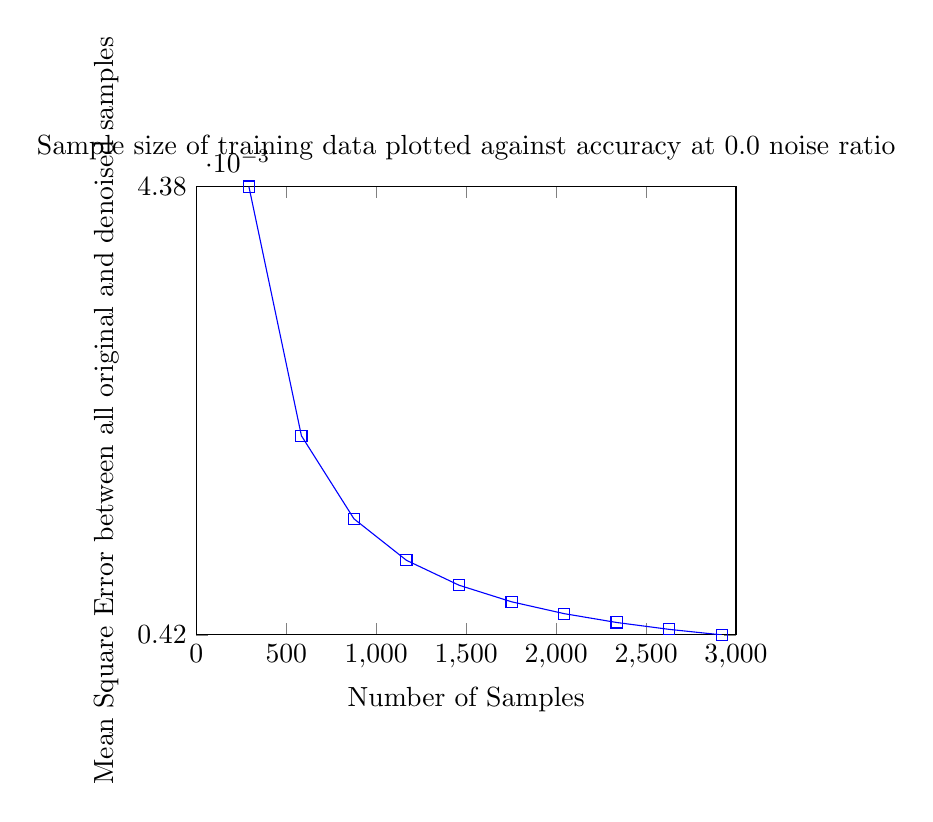
\begin{tikzpicture}
\begin{axis}[
title={Sample size of training data plotted against accuracy at 0.0 noise ratio},
xlabel={Number of Samples},
ylabel={Mean Square Error between all original and denoised samples},
xmin=0, xmax=3000,
ymin=0.0004187006744532279, ymax=0.004383824449905627,
xtick={0,500,1000,1500,2000,2500,3000},
ytick={0.0004187006744532279,0.004383824449905627},
legend pos=north west,
ymajorgrids=true,
grid style=dashed,
]

\addplot[
color=blue,
mark=square,
]
coordinates {

(292, 0.004383824449905627)
(584, 0.0021799053025073575)
(876, 0.001445356265023634)
(1168, 0.001078222616979597)
(1460, 0.0008581092100131867)
(1752, 0.0007114520790151598)
(2044, 0.0006068065606794189)
(2336, 0.0005284163200165668)
(2628, 0.00046750684177079003)
(2921, 0.0004187006744532279)
    };
\end{axis}
\end{tikzpicture}


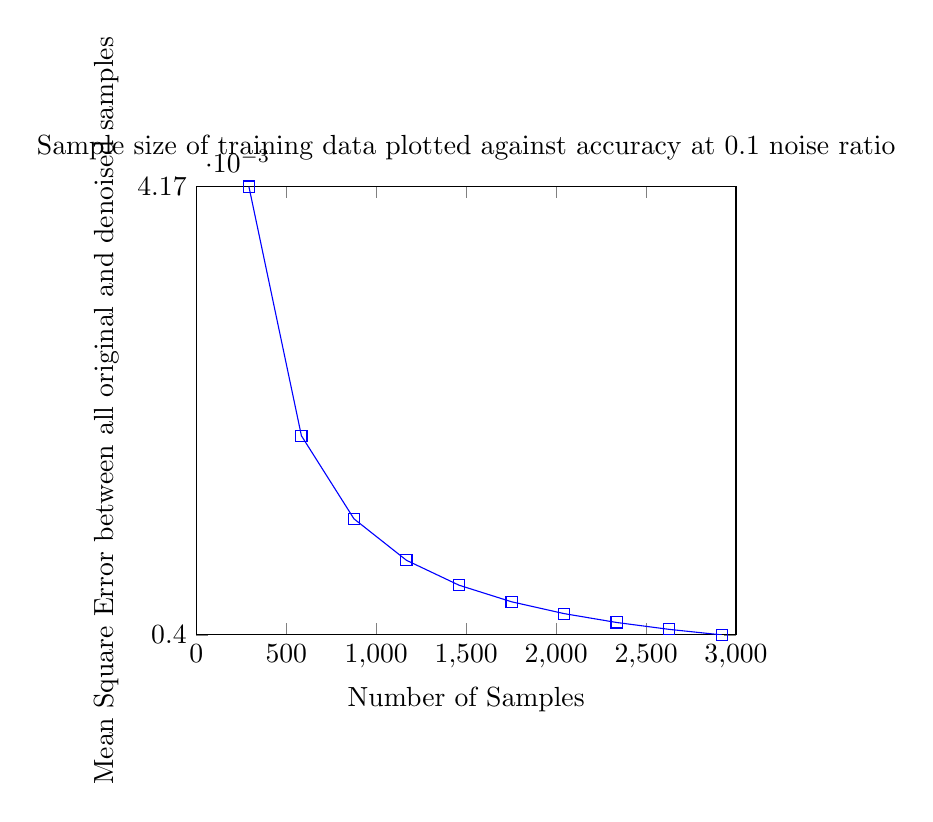
\begin{tikzpicture}
\begin{axis}[
title={Sample size of training data plotted against accuracy at 0.1 noise ratio},
xlabel={Number of Samples},
ylabel={Mean Square Error between all original and denoised samples},
xmin=0, xmax=3000,
ymin=0.00040275476849761685, ymax=0.0041699016718934065,
xtick={0,500,1000,1500,2000,2500,3000},
ytick={0.00040275476849761685,0.0041699016718934065},
legend pos=north west,
ymajorgrids=true,
grid style=dashed,
]

\addplot[
color=blue,
mark=square,
]
coordinates {

(292, 0.0041699016718934065)
(584, 0.0020759503972342533)
(876, 0.0013782160230494062)
(1168, 0.0010294869485192382)
(1460, 0.0008203636970436602)
(1752, 0.0006810422915765149)
(2044, 0.0005815946141254166)
(2336, 0.0005070752538567176)
(2628, 0.0004491736034707264)
(2921, 0.00040275476849761685)
    };
\end{axis}
\end{tikzpicture}

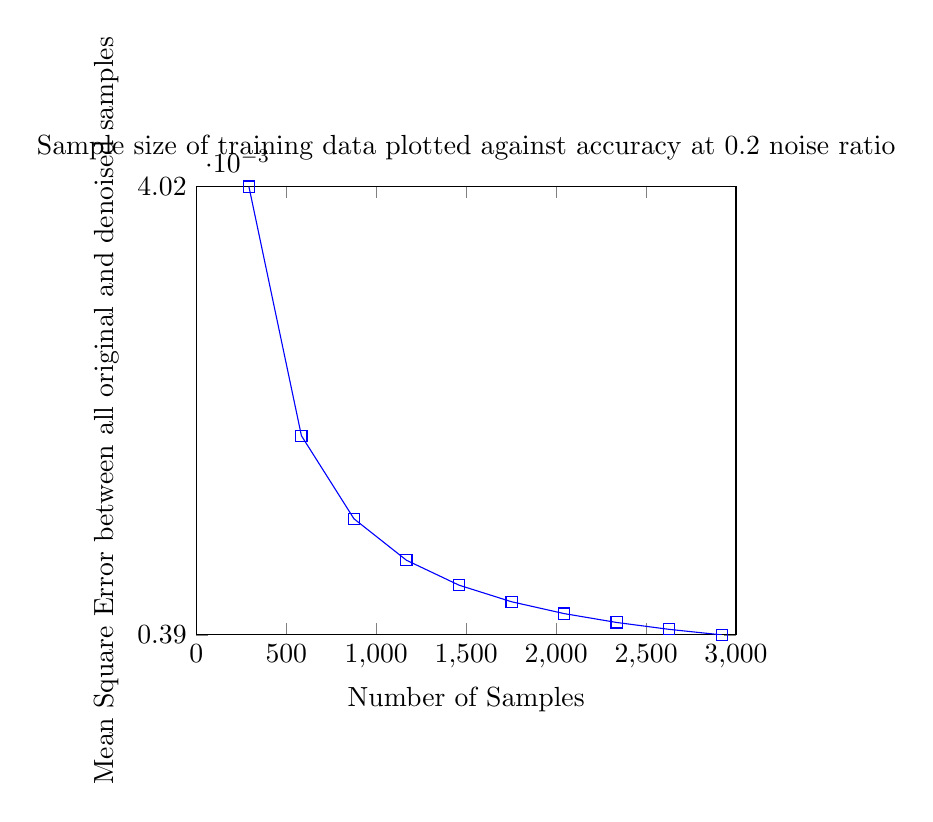
\begin{tikzpicture}
\begin{axis}[
title={Sample size of training data plotted against accuracy at 0.2 noise ratio},
xlabel={Number of Samples},
ylabel={Mean Square Error between all original and denoised samples},
xmin=0, xmax=3000,
ymin=0.00039149200964917264, ymax=0.004015853406190404,
xtick={0,500,1000,1500,2000,2500,3000},
ytick={0.00039149200964917264,0.004015853406190404},
legend pos=north west,
ymajorgrids=true,
grid style=dashed,
]

\addplot[
color=blue,
mark=square,
]
coordinates {

(292, 0.004015853406190404)
(584, 0.0020015835203805194)
(876, 0.001330320914188184)
(1168, 0.00099478954369694)
(1460, 0.0007935479691887362)
(1752, 0.0006594503124490673)
(2044, 0.0005637251739359213)
(2336, 0.0004919700827145676)
(2628, 0.0004362025751768176)
(2921, 0.00039149200964917264)
    };
\end{axis}
\end{tikzpicture}

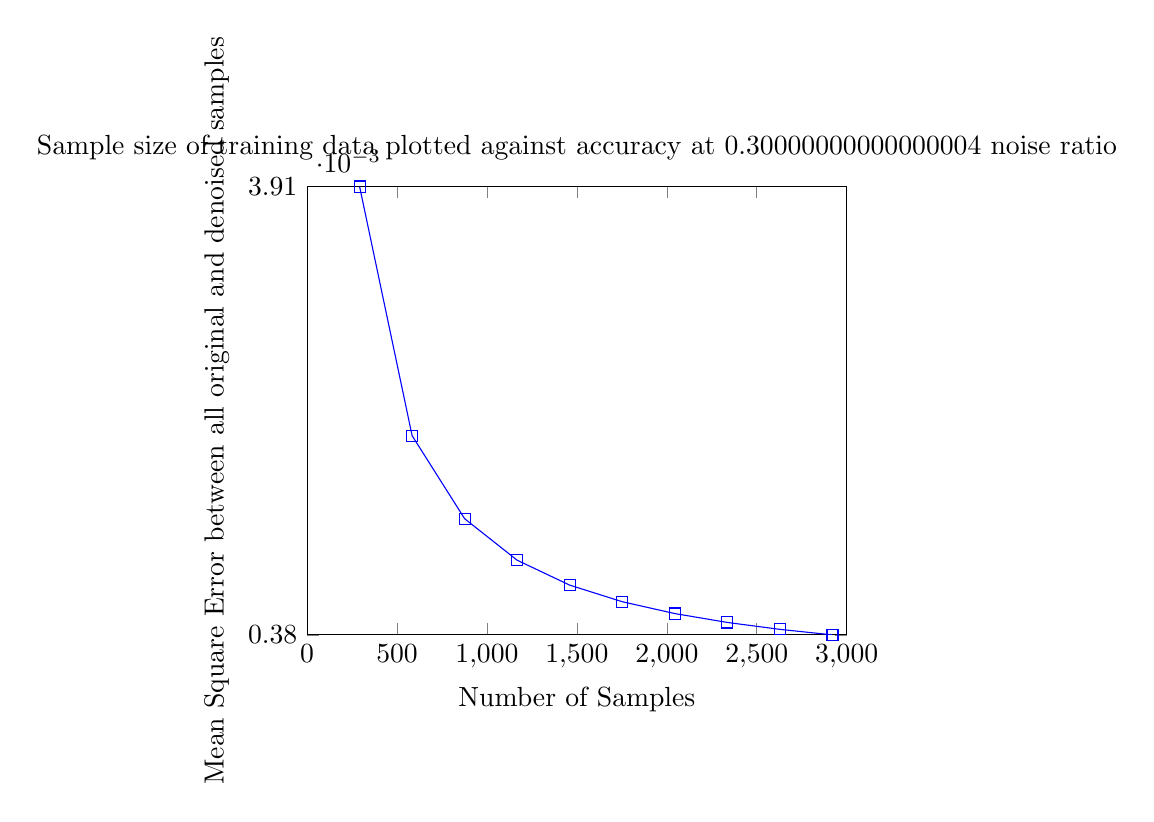
\begin{tikzpicture}
\begin{axis}[
title={Sample size of training data plotted against accuracy at 0.30000000000000004 noise ratio},
xlabel={Number of Samples},
ylabel={Mean Square Error between all original and denoised samples},
xmin=0, xmax=3000,
ymin=0.0003834001348172723, ymax=0.003906800916685965,
xtick={0,500,1000,1500,2000,2500,3000},
ytick={0.0003834001348172723,0.003906800916685965},
legend pos=north west,
ymajorgrids=true,
grid style=dashed,
]

\addplot[
color=blue,
mark=square,
]
coordinates {

(292, 0.003906800916685965)
(584, 0.0019488582890915718)
(876, 0.001296340325887012)
(1168, 0.0009701444427495749)
(1460, 0.0007744912473729393)
(1752, 0.0006440966683485644)
(2044, 0.0005509883974171702)
(2336, 0.00048118643150857896)
(2628, 0.00042691959492748363)
(2921, 0.0003834001348172723)
    };
\end{axis}
\end{tikzpicture}

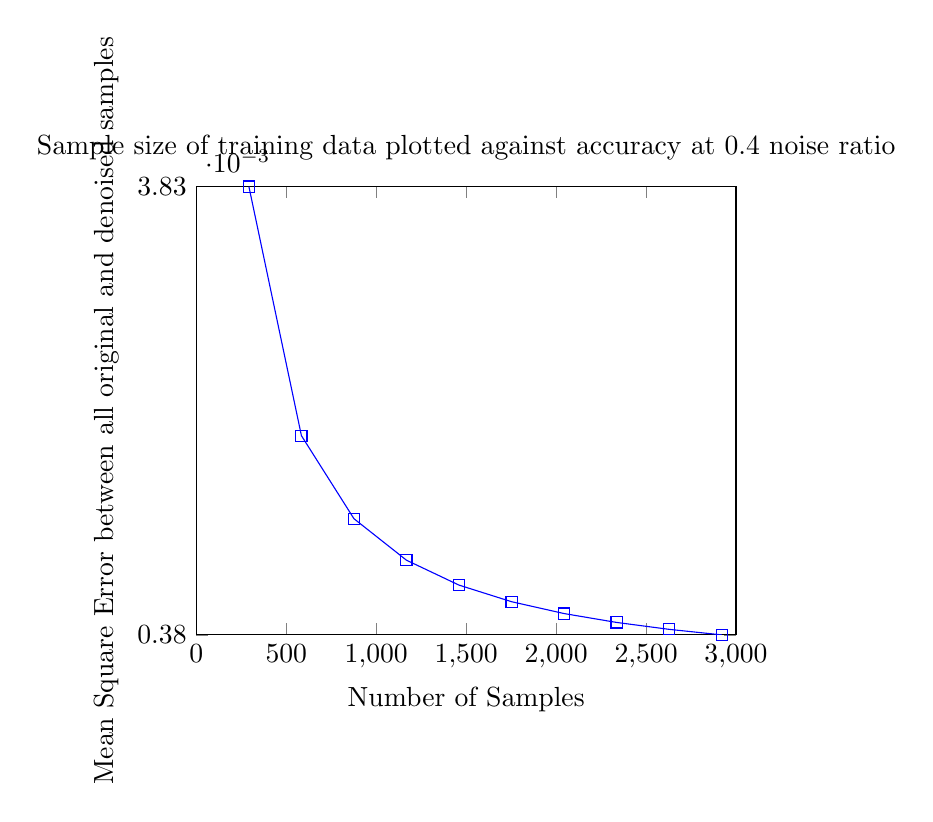
\begin{tikzpicture}
\begin{axis}[
title={Sample size of training data plotted against accuracy at 0.4 noise ratio},
xlabel={Number of Samples},
ylabel={Mean Square Error between all original and denoised samples},
xmin=0, xmax=3000,
ymin=0.0003774948390168696, ymax=0.0038285460717330257,
xtick={0,500,1000,1500,2000,2500,3000},
ytick={0.0003774948390168696,0.0038285460717330257},
legend pos=north west,
ymajorgrids=true,
grid style=dashed,
]

\addplot[
color=blue,
mark=square,
]
coordinates {

(292, 0.0038285460717330257)
(584, 0.0019110036460116926)
(876, 0.0012718814047235354)
(1168, 0.000952378350674965)
(1460, 0.0007607033223735599)
(1752, 0.0006329557452804532)
(2044, 0.0005417328886359958)
(2336, 0.00047333176033934434)
(2628, 0.0004201481742598481)
(2921, 0.0003774948390168696)
    };
\end{axis}
\end{tikzpicture}

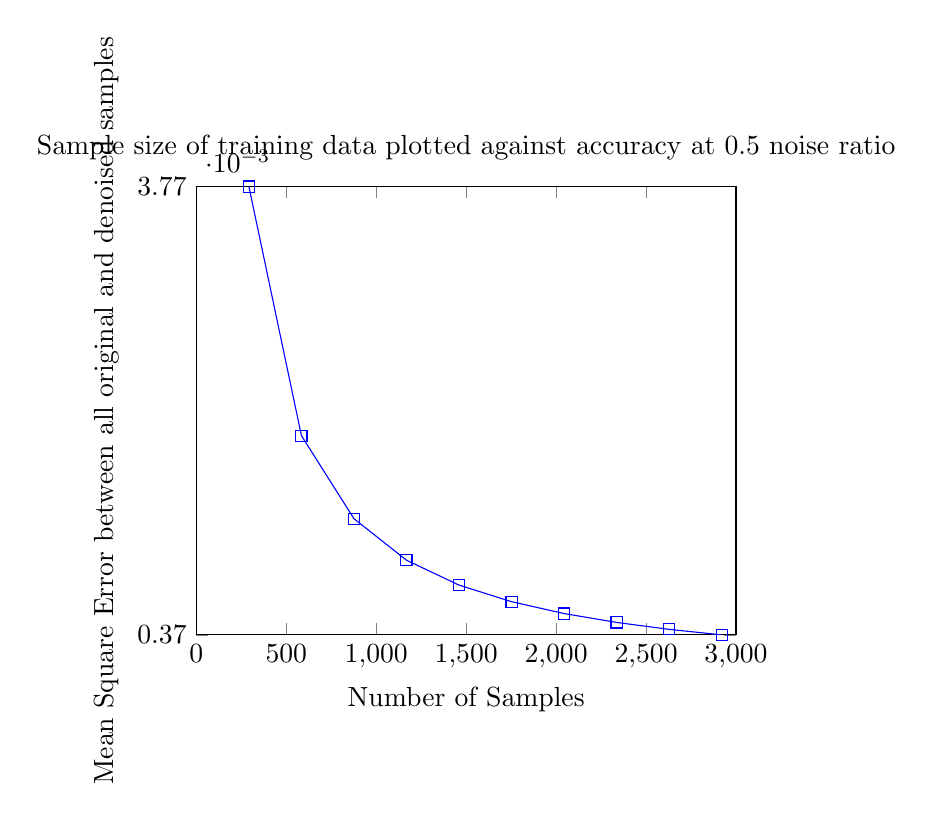
\begin{tikzpicture}
\begin{axis}[
title={Sample size of training data plotted against accuracy at 0.5 noise ratio},
xlabel={Number of Samples},
ylabel={Mean Square Error between all original and denoised samples},
xmin=0, xmax=3000,
ymin=0.00037307242246703245, ymax=0.0037711924675208775,
xtick={0,500,1000,1500,2000,2500,3000},
ytick={0.00037307242246703245,0.0037711924675208775},
legend pos=north west,
ymajorgrids=true,
grid style=dashed,
]

\addplot[
color=blue,
mark=square,
]
coordinates {

(292, 0.0037711924675208775)
(584, 0.0018831678337688997)
(876, 0.001253880203894581)
(1168, 0.0009392611027956084)
(1460, 0.0007505253845124269)
(1752, 0.000624710470871647)
(2044, 0.0005348641019620916)
(2336, 0.0004674938115088369)
(2628, 0.00041510251861484864)
(2921, 0.00037307242246703245)
    };
\end{axis}
\end{tikzpicture}

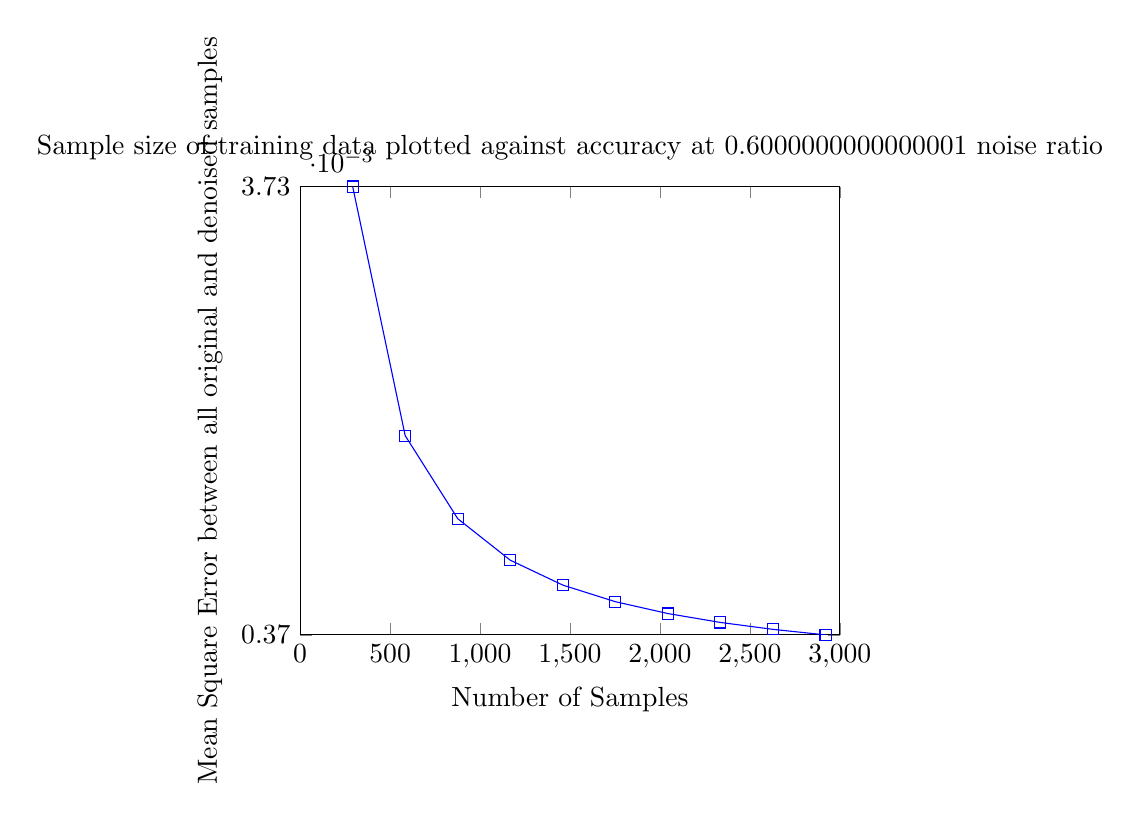
\begin{tikzpicture}
\begin{axis}[
title={Sample size of training data plotted against accuracy at 0.6000000000000001 noise ratio},
xlabel={Number of Samples},
ylabel={Mean Square Error between all original and denoised samples},
xmin=0, xmax=3000,
ymin=0.0003696846755190811, ymax=0.003728211107750603,
xtick={0,500,1000,1500,2000,2500,3000},
ytick={0.0003696846755190811,0.003728211107750603},
legend pos=north west,
ymajorgrids=true,
grid style=dashed,
]

\addplot[
color=blue,
mark=square,
]
coordinates {

(292, 0.003728211107750603)
(584, 0.001862261886104463)
(876, 0.0012403068013893232)
(1168, 0.0009293516864957806)
(1460, 0.0007427986181197255)
(1752, 0.0006184458250435452)
(2044, 0.0005296282232717134)
(2336, 0.0004630270903802918)
(2628, 0.0004112367120125105)
(2921, 0.0003696846755190811)
    };
\end{axis}
\end{tikzpicture}


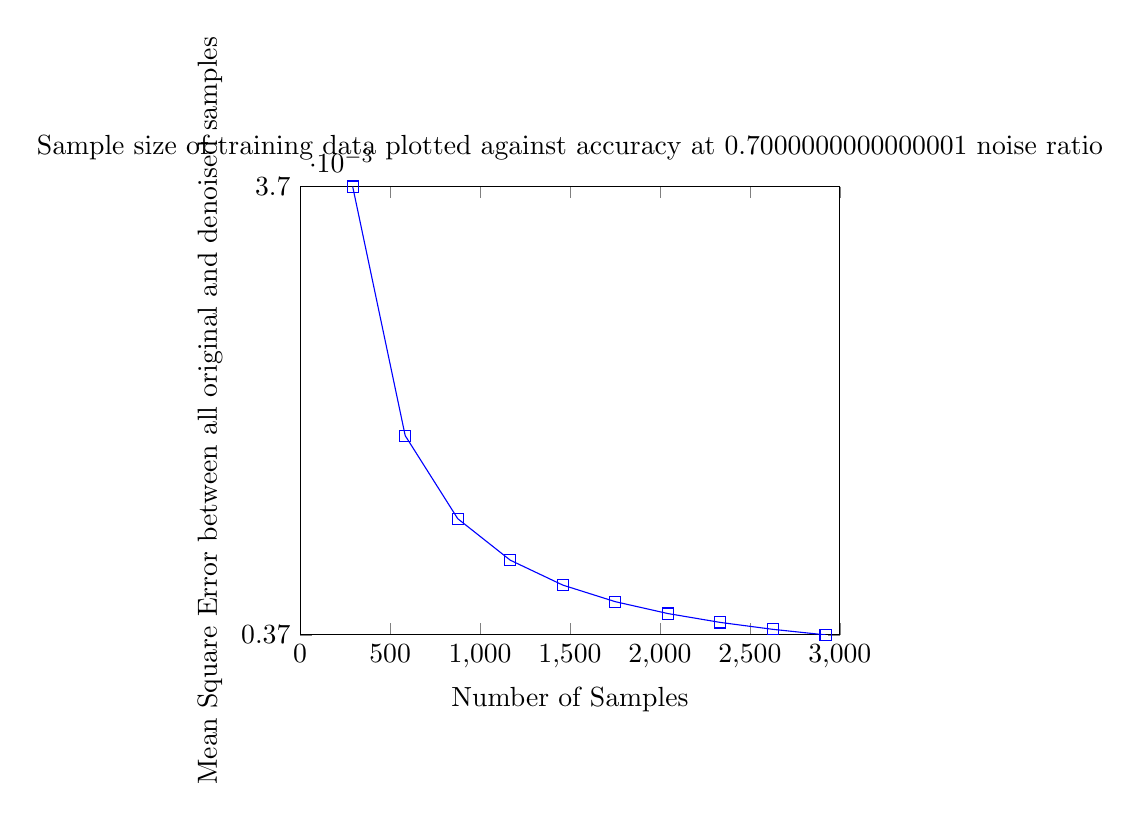
\begin{tikzpicture}
\begin{axis}[
title={Sample size of training data plotted against accuracy at 0.7000000000000001 noise ratio},
xlabel={Number of Samples},
ylabel={Mean Square Error between all original and denoised samples},
xmin=0, xmax=3000,
ymin=0.0003670268776127267, ymax=0.0036951730015683847,
xtick={0,500,1000,1500,2000,2500,3000},
ytick={0.0003670268776127267,0.0036951730015683847},
legend pos=north west,
ymajorgrids=true,
grid style=dashed,
]

\addplot[
color=blue,
mark=square,
]
coordinates {

(292, 0.0036951730015683847)
(584, 0.0018461456351439112)
(876, 0.0012298222297271433)
(1168, 0.0009216798939322338)
(1460, 0.0007368094472453019)
(1752, 0.0006135680695976376)
(2044, 0.000525549957603441)
(2336, 0.0004595440626924863)
(2628, 0.0004082130562101504)
(2921, 0.0003670268776127267)
    };
\end{axis}
\end{tikzpicture}


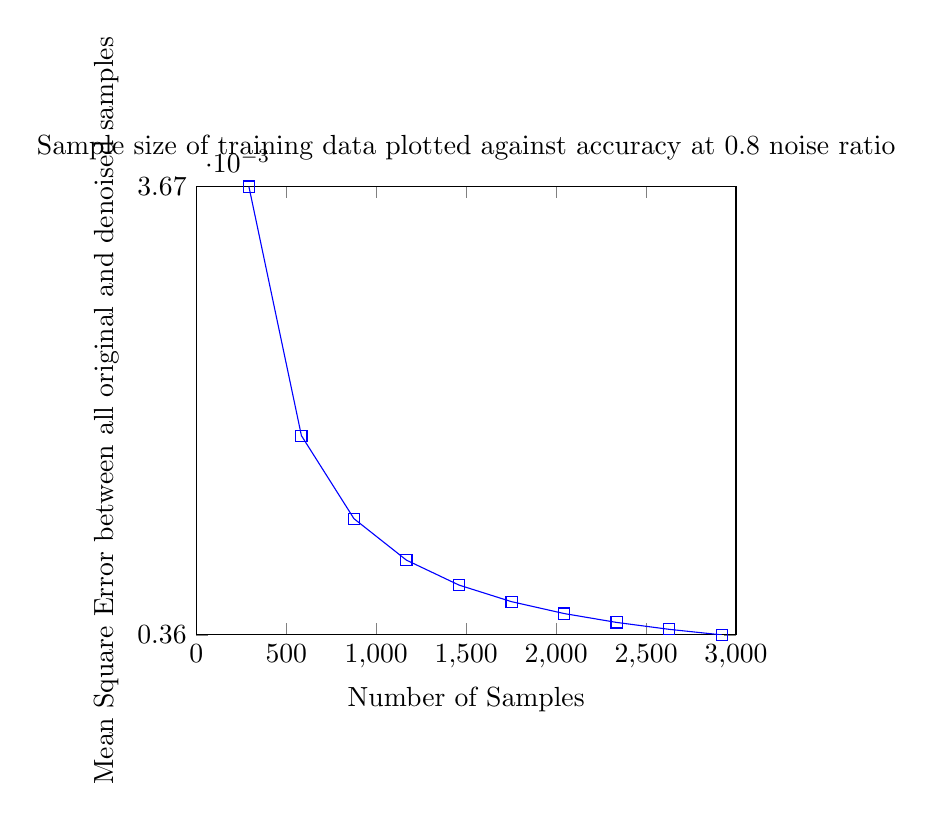
\begin{tikzpicture}
\begin{axis}[
title={Sample size of training data plotted against accuracy at 0.8 noise ratio},
xlabel={Number of Samples},
ylabel={Mean Square Error between all original and denoised samples},
xmin=0, xmax=3000,
ymin=0.00036490968731201477, ymax=0.0036692109277596655,
xtick={0,500,1000,1500,2000,2500,3000},
ytick={0.00036490968731201477,0.0036692109277596655},
legend pos=north west,
ymajorgrids=true,
grid style=dashed,
]

\addplot[
color=blue,
mark=square,
]
coordinates {

(292, 0.0036692109277596655)
(584, 0.001833459832560367)
(876, 0.0012215588077844459)
(1168, 0.0009156258097065684)
(1460, 0.0007320722613078091)
(1752, 0.0006097120486952076)
(2044, 0.0005223182604812324)
(2336, 0.00045677854782236974)
(2628, 0.0004058073103785003)
(2921, 0.00036490968731201477)
    };
\end{axis}
\end{tikzpicture}

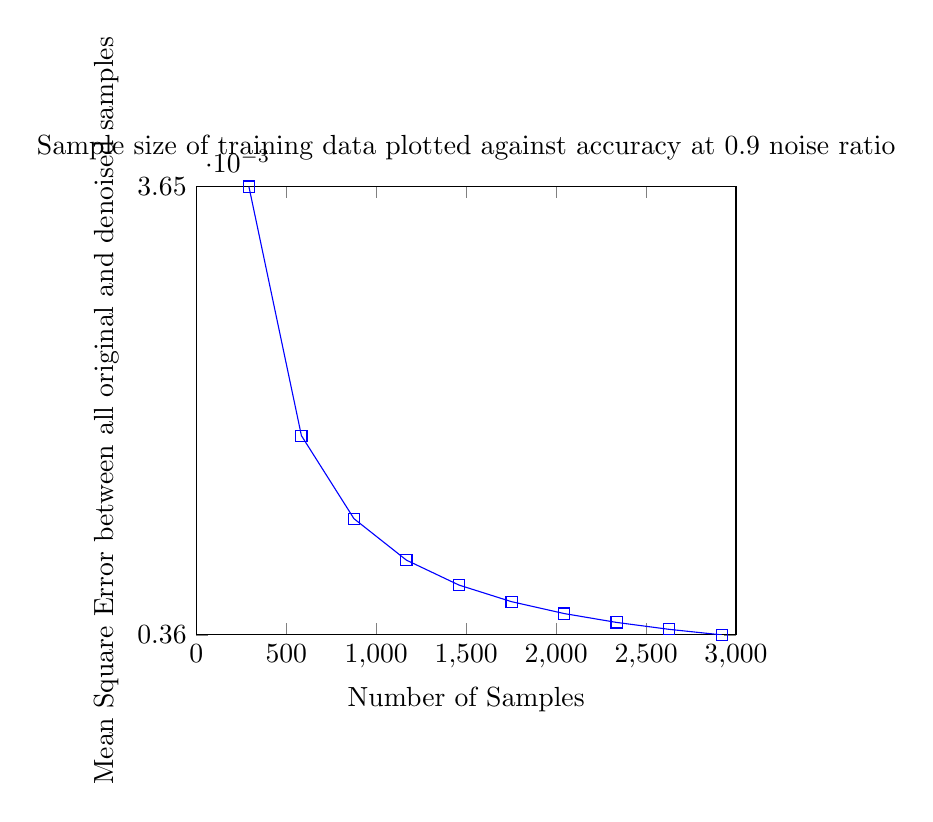
\begin{tikzpicture}
\begin{axis}[
title={Sample size of training data plotted against accuracy at 0.9 noise ratio},
xlabel={Number of Samples},
ylabel={Mean Square Error between all original and denoised samples},
xmin=0, xmax=3000,
ymin=0.00036317865549584117, ymax=0.003648412331610197,
xtick={0,500,1000,1500,2000,2500,3000},
ytick={0.00036317865549584117,0.003648412331610197},
legend pos=north west,
ymajorgrids=true,
grid style=dashed,
]

\addplot[
color=blue,
mark=square,
]
coordinates {

(292, 0.003648412331610197)
(584, 0.0018232758436105758)
(876, 0.00121491158151811)
(1168, 0.0009107383101503895)
(1460, 0.0007282446433422015)
(1752, 0.0006065879139719669)
(2044, 0.0005196925526069342)
(2336, 0.0004545260478506963)
(2628, 0.000403845546615584)
(2921, 0.00036317865549584117)
    };
\end{axis}
\end{tikzpicture}

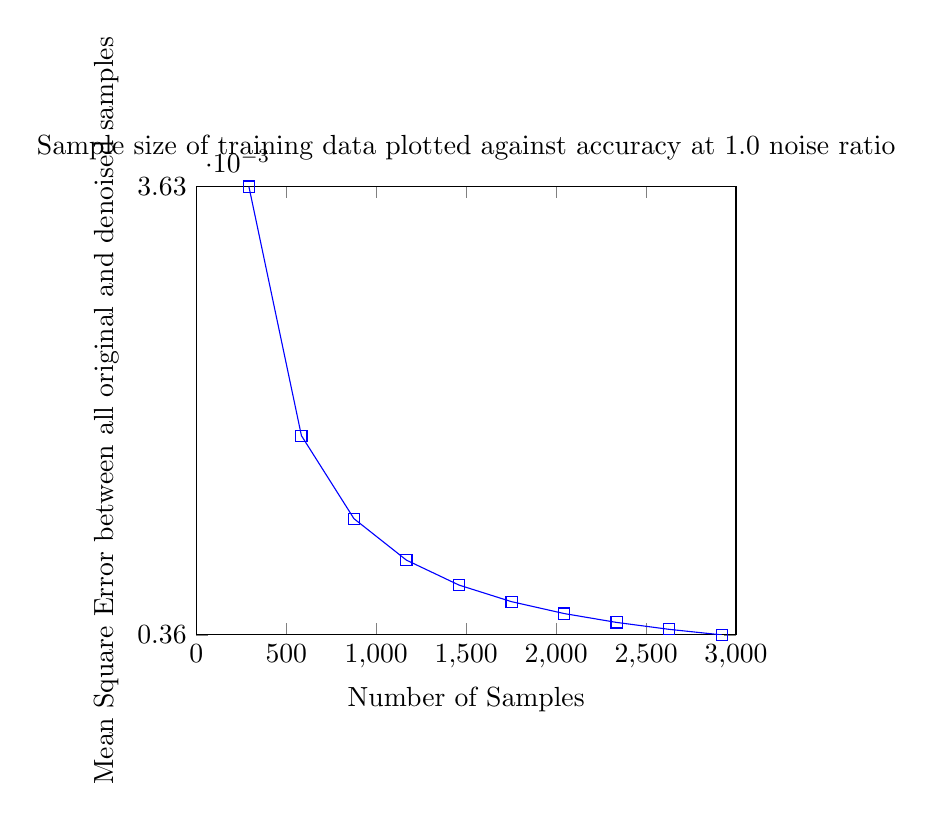
\begin{tikzpicture}
\begin{axis}[
title={Sample size of training data plotted against accuracy at 1.0 noise ratio},
xlabel={Number of Samples},
ylabel={Mean Square Error between all original and denoised samples},
xmin=0, xmax=3000,
ymin=0.0003617637972292147, ymax=0.0036315443316019486,
xtick={0,500,1000,1500,2000,2500,3000},
ytick={0.0003617637972292147,0.0036315443316019486},
legend pos=north west,
ymajorgrids=true,
grid style=dashed,
]

\addplot[
color=blue,
mark=square,
]
coordinates {

(292, 0.0036315443316019486)
(584, 0.0018150163343058781)
(876, 0.0012095145491585616)
(1168, 0.0009067714714062147)
(1460, 0.0007251356718665881)
(1752, 0.0006040452180967116)
(2044, 0.0005175558903706703)
(2336, 0.00045269020838515625)
(2628, 0.0004022432630742589)
(2921, 0.0003617637972292147)
    };
\end{axis}
\end{tikzpicture}


\end{document}